\documentclass[twoside,twocolumn,a4paper]{article}
\usepackage{EAAproceedings}

\begin{document}

% ****************  Begin of manuscript **********************
\Englishtitle{Modelling sound propagation in the presence of atmospheric 
turbulence for the auralisation of aircraft noise}

% Short title:
\Kolumnentitel{Rietdijk, Heutschi, Forssén: Atmospheric turbulence and aircraft auralisation} 

\PACS{43.28.Gq}

% 43.28.Gq	Outdoor sound propagation and scattering in a turbulent atmosphere, and in non-uniform flow fields
% 


% Authors' names, affiliations and addresses
% optionally grouped if with different institutions.
% First group:
\AuthorsI{Frederik Rietdijk, Kurt Heutschi}
\AddressI{Empa, Swiss Federal Laboratories for Materials Science and Technology, Dubendorf, Switzerland}
% Second group: (activate if applicable)
\AuthorsII{Jens Forssén}
\AddressII{Chalmers University of Technology, Gothenburg, Sweden}
% \AddressII{Chalmers University of Technology, Department of Civil \& Environmental Engineering, Gothenburg, Sweden}
% Third group (activate if applicable)
% \AuthorsIII{Maarten Hornikx}
% \AddressIII{Eindhoven University of Technology, Eindhoven, The Netherlands}


% English Abstract:
\Englishabstract{A new tool for the auralisation of aircraft noise in an urban 
environment is in development. When listening to aircraft noise sound level 
fluctuations caused by atmospheric turbulence are clearly audible. Therefore, to 
create a realistic auralisation of aircraft noise, the influence of atmospheric turbulence on sound propagation needs 
to be included. Presented is a model in development for including fluctuations due to 
movement through a frozen turbulent atmosphere in an auralisation.
}

% \abstract{
% A new tool for the auralisation of aircraft noise in an urban environment is in 
% development. When listening to aircraft noise sound level fluctuations caused by 
% atmospheric turbulence are clearly audible. Therefore, to create a realistic 
% auralisation of aircraft noise, atmospheric turbulence needs to be included.
% 
% Due to spatial inhomogeneities of the wind velocity and temperature in the 
% atmosphere acoustic scattering occurs, affecting the transfer function between 
% source and receiver. Both these inhomogeneities and the aircraft position are 
% time-dependent, and therefore the transfer function varies with time resulting 
% in the audible fluctuations. Assuming a stationary (frozen) atmosphere, the 
% movement of the aircraft alone gives rise to fluctuations.
% 
% Sound propagation of a moving source in a frozen atmosphere is simulated using a 
% k-space PSTD method. The impulse responses obtained from these simulations are 
% then used to create a simplified model describing the influence of turbulence on 
% a moving elevated source that can then be used to simulate the influence of 
% atmospheric turbulence in the auralisation of aircraft noise.
% }

\ScientificPaper
%newpage
\section{Introduction}
Aircraft noise can cause annoyance and sleep disturbance. Annoyance and
sleep disturbance is currently predicted using indicators based on time-averaged sound
pressure levels. This completely discards the character of the sound. To obtain a better 
representation of annoyance, the audible aircraft sound should be predicted in order to 
determine the impact of the sound on people.

Auralization is a technique to synthesise the aural aspects of an object or
surrounding. Auralization can therefore be used to create audible aircraft sounds that
can be used in listening tests.

\subsection{Aircraft auralisation tool}
An aircraft auralisation tool is being developed that should provide plausible 
auralisations of aircraft noise for typical urban situations where reflections 
and shielding can play an important role.

In the auralisation tool a distinction is made between a source model and a 
propagation model. The source model describes the emission of the aircraft, i.e. 
the spectral content as function of time and angle (directivity). 
The propagation model describes the propagation of the sound from source to receiver 
and currently supports:
\begin{itemize}
 \item spherical spreading resulting in a decrease of sound pressure with increase of source-receiver distance;
 \item Doppler shift due to relative motion between the moving aircraft and the non-moving receiver;
 \item atmospheric absorption due to relaxation processes;
 \item reflections at the ground and facades.% due to a sudden change in impedance;
\end{itemize}
The propagation model is based on geometrical acoustics. The reflections are determined using the Image Source Method.

\subsection{Turbulence}
When listening to aircraft noise, sound level fluctuations caused by atmospheric 
turbulence are clearly audible. Therefore, to create a realistic auralisation of 
aircraft noise, atmospheric turbulence needs to be included.

Due to spatial inhomogeneities of the wind velocity and temperature in the atmosphere, 
acoustic scattering occurs, affecting the transfer function between source and receiver. 
Both these inhomogeneities and the aircraft position are time-dependent, and therefore 
the transfer function varies with time resulting in the audible fluctuations. 

The theory of turbulence is a statistical theory. A statistical theory fits well 
with the physics of turbulence since turbulence is a consequence of instability of 
fluid flow in relation to very small fluctuations in the fluid \cite{Tatarskii1971}. For an auralisation instantaneous values of the sound pressure at the receiver are required.

Artnzen\cite{Arntzen2013a} included a phase fluctuations filter in their aircraft noise simulator to make the ground effect less pronounced.
The filter was based on a Gaussian spectrum of turbulence.

In this paper an initial model is presented to describe fluctuations in the sound pressure due to atmospheric 
turbulence as function of time. A stationary (frozen) atmosphere is assumed where the 
movement of the aircraft alone gives rise to fluctuations.
In contrast to Arntzen\cite{Arntzen2013a}, both amplitude and phase fluctuations are considered. The model is based on a simple model by Daigle et. al.\cite{Daigle1983}.


\section{Theory}
As mentioned in the introduction the theory of turbulence is a statistical theory.
The wind velocity components and temperature in the turbulent atmosphere are fluctuating functions of both position and time.

% \subsection{Correlation function}
The fields of the wind velocity components and the temperature are random fields.
A characteristic of a random function or field is it's correlation function. \cite{Tatarskii1971}
The correlation function of such a random field $f(\mathbf{r})$, as function of distance $\mathbf{r}$ between observation points only, is defined as
\begin{equation}
 B(\mathbf{r}_1, \mathbf{r}_2) = \langle f(\mathbf{r}_1  f(\mathbf{r}_2) \rangle
\end{equation}
Note that we've assumed a 'frozen turbulence' here. 

In a homogeneous and isotropic random field the correlation function $B(\mathbf{r})$ 
depends only on $|r|=\mathbf{r}$, i.e., only the distance between the observation points.


\subsection{Gaussian spectrum}
In the region of large eddy sizes the turbulence spectrum can be approximated by a Gaussian distribution.
The spatial correlation function for the fluctuating refractive-index $\mu$ therefore also has a Gaussian form
\begin{equation}
 \langle \mu_1 \mu_2 \rangle = \langle \mu^2 \rangle \exp{\left( -x^2 / L^2 \right)}
\end{equation}
When the outer length scale of the turbulence $L$ is much smaller than the Fresnel zone, 
the mean square log-amplitude and phase fluctuations for spherical waves are given by
\begin{equation}\label{eq:model_daigle}
 \langle \chi^2 \rangle = \langle S^2 \rangle = \frac{\sqrt{\pi}}{2} \langle \mu^2 \rangle k^2 r L 
\end{equation}
where $k$ is the wavenumber and $r$ is the distance of propagation.
The mean square log-amplitude and phase fluctuations are defined respectively as $\langle \chi^2 \rangle = \langle \left( \ln{\frac{A_{n}}{A_{m}}} \right) ^2 \rangle $
and $ \langle S^2 \rangle = \langle \left( \phi_n - \phi_m \right)^2  \rangle$. The index $n$ indicates the sample $n$ at time $t$ and index $m$ the average fluctuation.
For spherical waves the covariances of the fluctuations, $B_{\chi}(\rho)$ and $B_{S}(\rho)$, normalized to their variances, are given by
\begin{equation}
 \frac{B_{\chi} (\rho)}{\langle \chi^2 \rangle} = \frac{B_{S} (\rho)}{\langle S^2 \rangle} = \frac{\Phi\left(\rho/L\right)}{\rho/L}
\end{equation}
where 
\begin{align}
 \phi \left(\rho/L \right) &= \int_0^{\rho/L} \exp{\left(-u^2\right)} \mathrm{d} u 
 &= \frac{1}{2} \sqrt{\pi} \mathrm{erf}\left( \rho/L \right)
\end{align}
with $\mathrm{erf}$ the error function.
The covariance of the fluctuations $B_{\chi}(\rho)$ and $B_{S}(\rho)$ are thus given by
\begin{equation}
 B_{\chi} (\rho) = B_{S}(\rho) = \frac{\sqrt{\pi}}{2}  \langle \mu^2  \rangle k^2 r L 
\frac{\Phi(\rho/L) }{\rho / L}
\end{equation}
according to Daigle's model.

\subsection{Time series of fluctuations}
% The fluctuations of the random fields cause amplitude and phase fluctuations or modulations.
For the auralisation, time series of instantaneous fluctuations of log-amplitude and phase are required, $\chi(t)$ and $S(t)$.
Because the modulations are frequency-dependent, we would like to obtain realisations of $\chi(t, f)$ and $S(t, f)$ which describe the fluctuation of the log-amplitude $\chi$ and phase $S$ at a time $t$ for frequency $f$.
The frequency $f$ is the frequency of the signal component that should be modulated.

By assuming that $\chi(t,f)$ and $S(t,f)$ are Gaussian random variables, we can produce realisations of $\chi(t,f)$ and $S(t,f)$ by filtering white noise with a chosen filter function.
The desired filter response is the impulse response $h(\rho)$ of the covariance $B(\rho)$, which is obtained by taking the inverse Fourier transform of the square root of the autospectrum of $B(\rho)$.
% \begin{equation}
%  h(\rho) = \sqrt{S_{\rho}}
% \end{equation}

By taking these steps, two series of fluctuations are obtained, $\chi(t, f)$ and $S(t, f)$. 
The two time series can be merged into a single complex modulation signal
\begin{equation}
 m(t,f) = \exp{\left( \chi\left(t,f\right) + j S\left(t, f\right) \right)}
\end{equation}
that can then be applied to the input signal.

\subsection{Saturation of the log-amplitude}
For longer path lengths and stronger turbulence, the amplitude fluctuations gradually level off.
Saturation of the amplitude fluctuations can be observed when measuring aircraft noise at distances of over a few kilometers.
The standard deviation of the fluctuating sound pressure levels is in such cases limited to no approximately 6 dB \cite{Daigle1983,Piercy1974}.

Saturation of the log-amplitude can be included based on an analysis by Wenzel \cite{Wenzel1975}.
In Wenzel's approach the soundwave is split up in a coherent and incoherent wave. The amplitude of the coherent wave decreases over distance while the incoherent wave obtains the energy from the coherent wave.
The coherent wave $p$ is written as
\begin{equation}
 \langle p \  p^* \rangle = \left( A_m^2 / 4 \pi r^2 \right) \exp{\left( -2 \langle \mu^2 \rangle k^2 r L \right)}
\end{equation}
Wenzel defines the distance to saturation $r_s$ as the distance at which the coherent wave is reduced to $e^{-1}$ of its original strength
\begin{equation}\label{eq:saturation_distance}
 r_s = \frac{1}{2 \langle \mu^2 \rangle k^2 L}
\end{equation}
Saturation of the log-amplitude fluctuations can now be included by multiplying $\chi(t,f)$ with
\begin{equation}
 \sqrt{ \frac{ 1}{1 + r/r_s}}
\end{equation}


\subsection{Applying the modulations to the original signal}
In case the input signal consists of just one frequency $f$ and the modulation 
signal $m$ is calculated for that specific frequency, then the modulation can simply be 
applied by multiplying the two in the time-domain.
However, for the auralisation we have broadband sounds with more than one frequency line to consider. 
As the fluctuations are frequency-dependent, the modulation 
signal would have to be calculated for every frequency line.

One of the design criteria of the auralisation tool is to produce at or near 
real-time auralisations. Since computing the modulation signal for every 
frequency line is computationally relatively heavy, another solution is sought.
The variances of the log-amplitude and phase fluctuations increase according to 
this simple theory linearly with frequency. Therefore, another option would be to scale both 
$\chi(t,f)$ and $S(t,f)$ accordingly. Care should be taken considering the saturation distance is frequency-dependent.






% % To obtain the modulation spectrum the following steps are performed:
% % 
% % \begin{enumerate}
% %  \item Sample the correlation function $B(\rho)$ at distances $\rho_m$ where $\Delta \rho$ is small enough to resolve the acoustic field.
% %  \item Optionally apply a window.
% %  \item Fourier transform and calculate the autospectrum $C_{xx}$.
% %  \item Inverse Fourier transform of the square root of the autospectrum.
% %  \item $C_{xx}$ to obtain $h(\rho_m)$.
% %  \item Convolute $h(\rho_m)$ with white noise to obtain the fluctuations $\chi$ and $S$.
% %  \item Modulation spectrum $M(f)$ is then given by $M(f) = e^{\chi(y_i) + j S(y_i)} \cdot e^{-B(0)}$
% % \end{enumerate}
% % 
% % 
% % The modulation spectrum can then be applied to the acoustic signal $p$.
% % 
% % \begin{enumerate}
% %  \item Inverse Fourier transform of the modulation spectrum $M(f)$ to obtain the modulation impulse response $m(t)$.
% %  \item Resample the impulse response $m(t)$ to match with the sample frequency of the acoustic signal $p(t)$.
% %  \item Perform the convolution between the acoustic signal $p(t)$ and the modulation impulse response $m(t)$.
% % \end{enumerate}
% % 
% % The log-amplitude and phase fluctuations are described by
% % \begin{align}
% %  \chi &= \log{A / A_0} \\
% %  S &= \phi - \phi_0
% % \end{align}
% % where $A$ and and $\phi$ are respectively the amplitude and phase in presence of turbulence and 
% % $A_0$ and $\phi_0$ respectively the amplitude and phase in absence of turbulence.
% %  
% % The correlation function for the log-amplitude and phase fluctuations can be written respectively as
% % \begin{align}
% %   B_{\chi} \left( \rho \right) &= \langle \chi (\mathbf{r}), \chi( \mathbf{r}+\mathbf{\rho} ) \rangle \\
% %   B_S \left( \rho \right) &= \langle S (\mathbf{r}), S( \mathbf{r}+\mathbf{\rho} ) \rangle
% % \end{align}
% % where $\mathbf{r}$ describes a point in the field and $\mathbf{\rho}$ is a transversal separation from the point $\mathbf{r}$.
% % 
% % 
% % For a Gaussian model
% % \begin{equation}
% %  B_{\chi} ( \rho ) = B_{S} ( \rho ) = \mu_0^2 k^2 L l .....
% % \end{equation}
% % 
% %  
% % Realisations of the log-amplitude and phase fluctuations are then produced by the convolution of 
% % $h\left(\rho_m \right)$ and Gaussian white noise with a mean value of 0 and variance 1.
% % 
% % The modulation signal is calculated for a single frequency $f_m$.
% % Higher frequencies are affected more strongly by turbulence.


% For every frequency in the input signal the modulation signal is applied albeit with a different multiplication.
% 
% The modulated signal is then calculated as
% % \begin{equation}
% %  \hat{p}_{out} = \sum_{i=0}^n \Re{A[i] exp{j \omega t} f_m}
% % \end{equation}
% 
% 
% 
% The following procedure can be followed as well for other turbulence models, e.g. the Von Karman model.
% 
% Since the modulation spectrum is range dependent it should eventually be 
% calculated for every source-receiver distance.


% See BAC 8.54. Scattered power relative to free field is proportional to $f^{1/3}$


% 
% \subsection{Time-domain simulations}
% 



\section{Results}
An example of a calculated modulation signal $m(t,f)$ caused by fluctuations of the refractive-index in a Gaussian field is shown in figure \ref{fig:modulation_signal}.
The figure shows the log-amplitude and phase fluctuations as function of time for a specific frequency.
% For this example the mean squared refractive-index is $\mu = 3 \cdot 10^{-6}$, the outer length scale $L = 15 $ m, speed of sound $c=343$ m/s, and the distance $r$ 2000 meters. 
% The sample frequency is 10000 Hz and duration of the fragment is 10 seconds.

\Figure{fig:modulation_signal}{Amplitude and phase fluctuations as function of time for 200 Hz. The parameters $\langle \mu^2 \rangle = 3 \cdot 10^{-6}$, $L = 15 $ m, $c=343$ m/s, $r=2000$ m, were used.}
       {60}{ \put(3,3)  {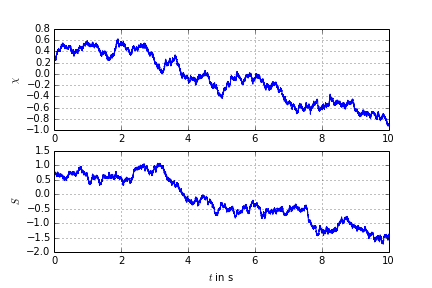
\includegraphics[width=75mm]{../figures/modulation_signal}}}

To check whether the resulting variance of the log-amplitude and phase fluctuations of such a modulation signal are as they should be, a comparison is made with equation \ref{eq:model_daigle}.
The extraction and analysis of the mean square amplitude and phase fluctuations follows the method of Daigle et al.

The mean square log-amplitude fluctuation was calculated as
\begin{equation}
 \langle \chi^2 \rangle = \frac{1}{N} \sum_{n=1}^N \chi_n^2
\end{equation}
where
\begin{equation}
 \chi_n = \ln{\left(A_n/A_m\right)}
\end{equation}
and $A_m$ is the average amplitude over $N$ samples in time
\begin{equation}
 A_m = \frac{1}{N} \sum_{n=1}^N A_n
\end{equation}
where $n$ is the sample at time $t$. Similarly, the mean square of the phase fluctuations is calculated as
\begin{equation}
 \langle S^2 \rangle = \frac{1}{N} \sum_{n=1}^N \left( \phi_n - \phi_m \right)^2
\end{equation}
with
\begin{equation}
 \phi_m = \frac{1}{N} \sum_{n=1}^N \phi_n
\end{equation}


Figure \ref{fig:function_of_frequency} shows the log-amplitude and phase variances as function of frequency. The frequency-dependency is maintained although the variance is slightly lower than expected.

\Figure{fig:function_of_frequency}{Log-amplitude and phase variances as function of frequency. The parameters $\langle \mu^2 \rangle = 3\cdot 10^{-6}$, $L=15$ m, $c=343$ m/s, $r=2000$ m, were used.}
       {60}{ \put(3,3)  {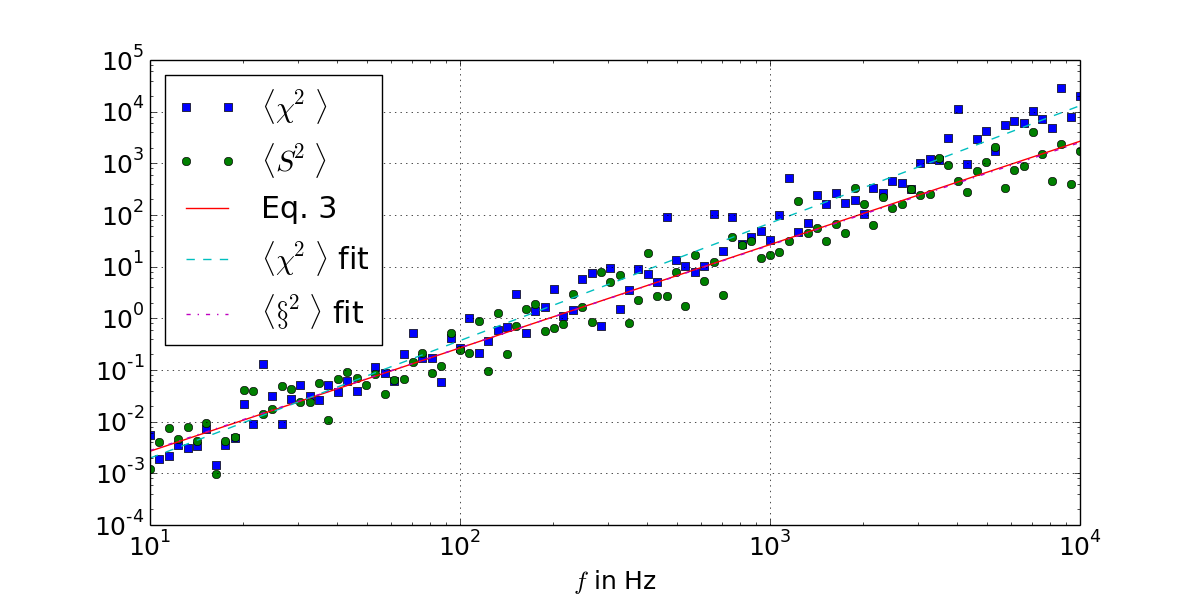
\includegraphics[width=75mm]{../figures/function_of_frequency}}}
       
The same applies to the distance-dependency. Figure \ref{fig:function_of_distance} shows the log-amplitude and phase variances as function of distance. The variance of the fluctuations is also slightly lower than expected.
       
\Figure{fig:function_of_distance}{Log-amplitude and phase variances as function of distance. The parameters $\langle \mu^2 \rangle = 3\cdot 10^{-6}$, $L=15$ m, $c=343$ m/s, $f=200$ Hz, were used.}
       {60}{ \put(3,3)  {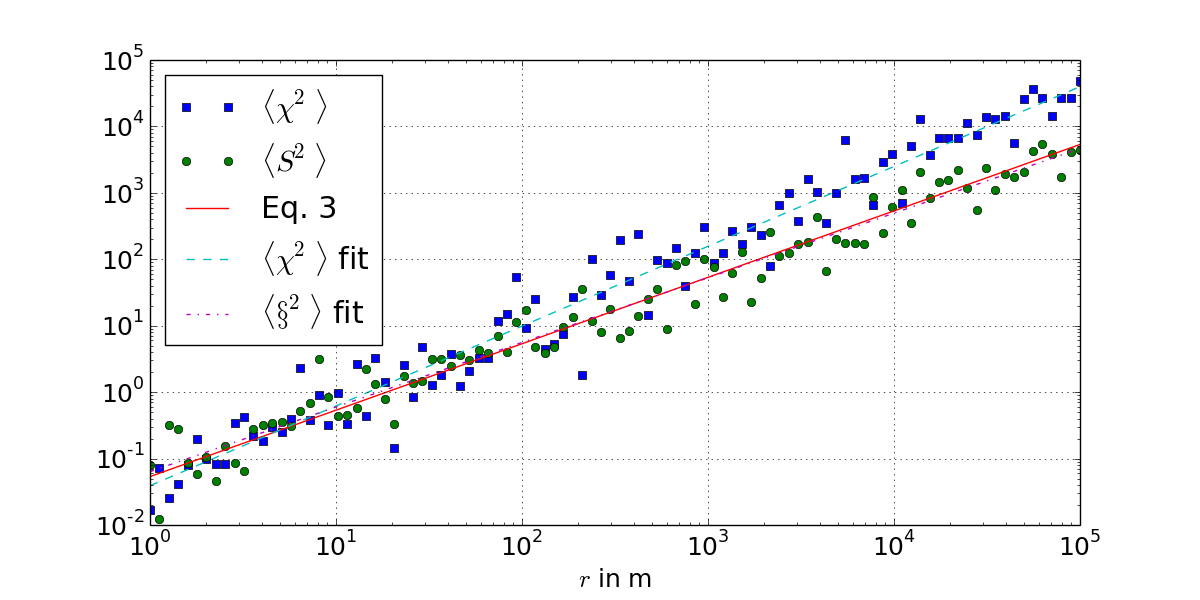
\includegraphics[width=75mm]{../figures/function_of_distance}}}
       
While the simple theory predicts that the mean square log-amplitude and phase fluctuations are equal, Daigle et. al. \cite{Daigle1983} showed through measurements that the log-amplitude fluctuations don't obey the simple theory but are in fact smaller than predicted.
Figure \ref{fig:function_of_distance_with_saturation} shows again the mean square fluctuations as function of distance, but this time taking into account log-amplitude saturation.

\Figure{fig:function_of_distance_with_saturation}{Log-amplitude and phase variances as function of distance taking into account the log-amplitude saturation. 
The same parameters as in \ref{fig:function_of_distance} were used. The distance to saturation $r_s$, calculated using equation \ref{eq:saturation_distance}, was 827 m.}
       {60}{ \put(3,3)  {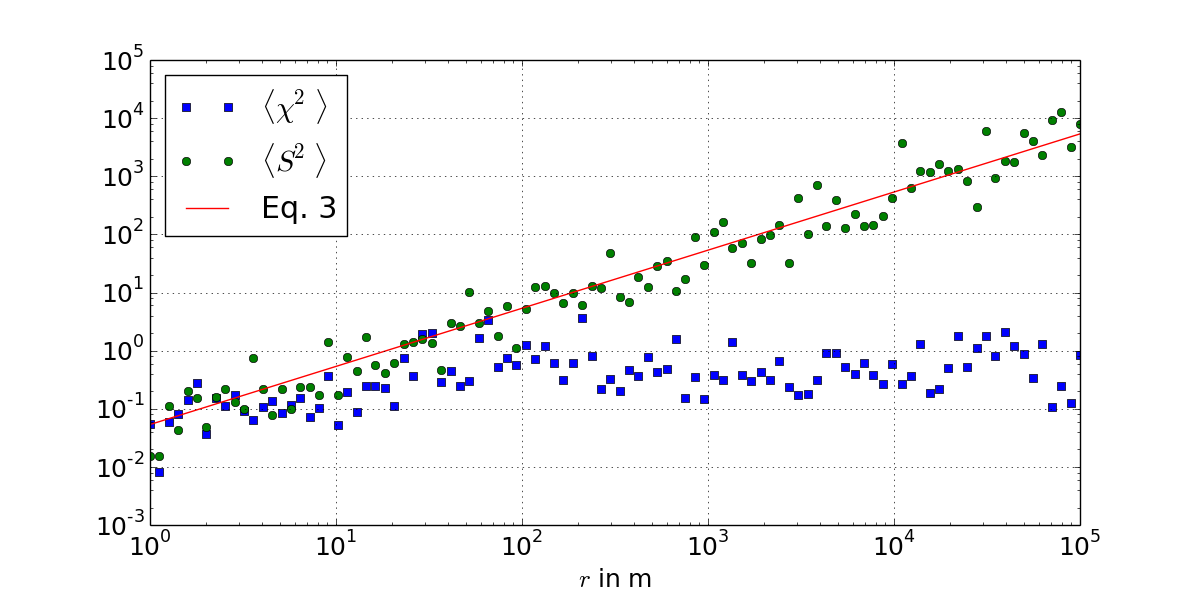
\includegraphics[width=75mm]{../figures/function_of_distance_with_saturation}}}


Finally, the modulation signal was applied to a tone of the same frequency as the modulation signal was calculated for. The resulting signal is shown in figure \ref{fig:levels}.
\Figure{fig:levels}{Sound pressure level $L_p$ of a signal modulated by the modulation signal shown in figure \ref{fig:modulation_signal}.
The input signal is a sine wave of 200 Hz. Time-weighting 'F' was used. The standard deviation of this modulated signal is 7 dB.}
       {60}{ \put(3,3)  {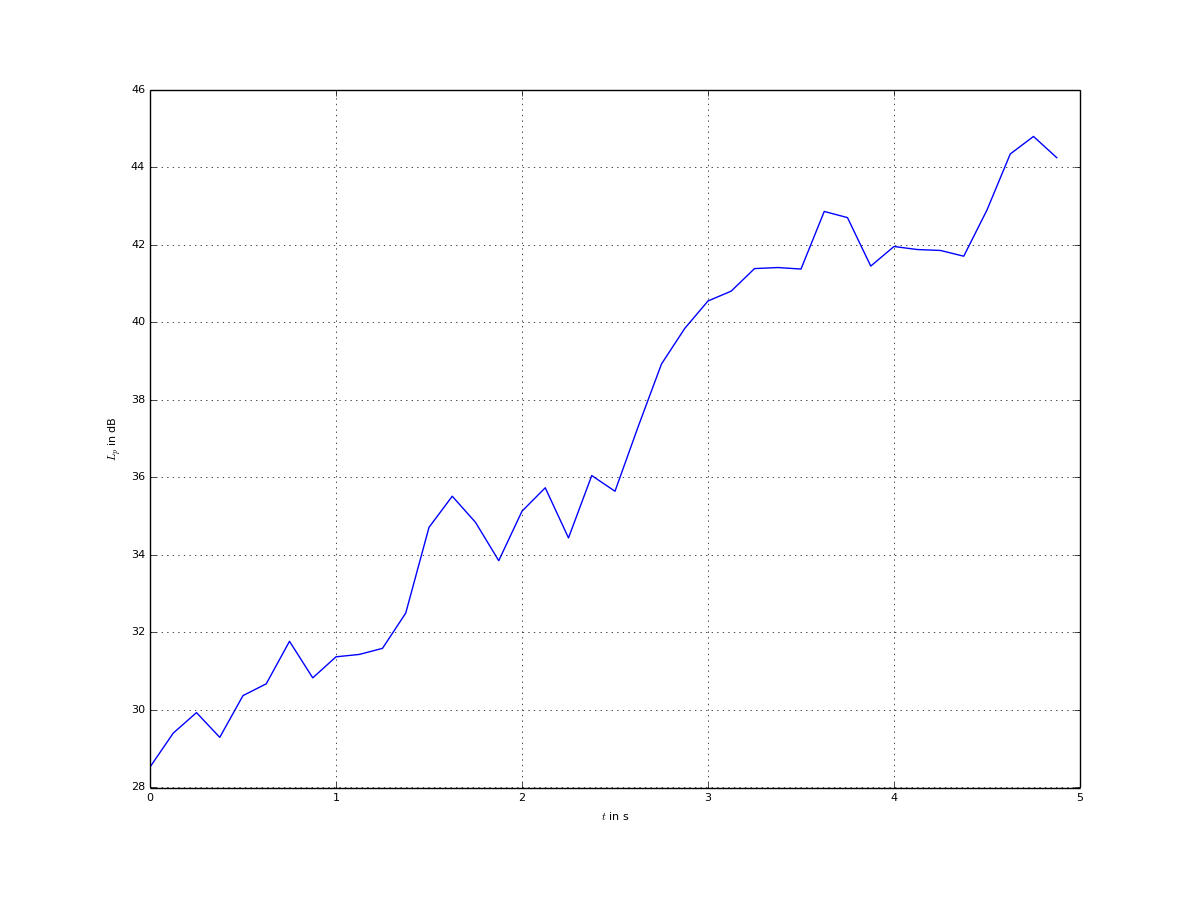
\includegraphics[width=75mm]{../figures/levels}}}

\section{Discussion}
Based on a simple theory presented by Daigle et. al. a method is described to include modulations due to turbulence in an auralisation.
The mean square of the fluctuations seem to be slightly smaller than what can be expected from the theory. It is not known why.

An important limitation of the current model is the fact that the turbulence is assumed to be homogeneous and isotropic, which means the height-dependency of the turbulence due to the boundary conditions is ignored.
% \subsection{Height-dependency}
% First of all, by assuming that the turbulence can be considered homogeneous and 
% isotropic the height-dependency of the turbulence due to the boundary conditions is ignored.
The outer length scale of the turbulence is known to increase with height, as can be seen in 
vertical profiles of the outer scale of turbulence obtained through acoustical sounding by Krasnenko et. al.\cite{Krasnenko2013}.

Also, it is assumed that the outer length scale of the turbulence is much smaller than the Fresnel zone. When the aircraft is directly above the receiver and at relatively low altitude, this assumption will not be valid either.
For example, at an altitude of 200 meters and a frequency of 100 Hz the Fresnel zone is 7.6 meters. The outer length scale is however in the order of 10 meters.

Figure \ref{fig:levels} shows the sound pressure level as function of time of a signal modulated using the presented method.
It should be noted that it is a mere coincidence that the standard deviation is similar to that what is expected at such distances.
More calculations and with longer averaging times need to be done to determine what the standard deviation is after saturation of the log-amplitude.

% For longer averaging times the standard deviation of the level fluctuations seems to level out at 9 dB instead.
In a next step k-space PSTD time-domain simulations will be performed as well to determine saturation distances and standard deviations of the level fluctuations after saturation of the log-amplitude.
These simulations should also reveal more information regarding the coherence of the fluctuations between different frequencies.


% \subsection{Limitations of the model}
% \begin{enumerate}
%  \item The turbulent boundary layer is ignored. While turbulence is height dependent a homogeneous and isotropic turbulence is assumed. 
%  \item (However, the fluctuations are mainly determined close to the source. A height dependent outer length scale is therefore perhaps not that important? Needs reference.)
%  \item In certain positions the outer length scale of the turbulence might not be much smaller than the Fresnel zone. 
% %  \item Lack of amplitude saturation.
% %  \item (Saturation of the log-amplitude can be prevented by having a height-dependent modulation depth?)
% \end{enumerate}


\section{CONCLUSIONS}
A method is presented to include modulations caused by turbulence in an auralisation.
The model is based on a simple theory assuming a Gaussian spectrum. The saturation of log-amplitude fluctuations is explicitly included in the model.
Future work includes comparisons with time-domain simulations of sound propagation through a turbulent atmosphere.


\Acknowledgement{The research leading to these results has received funding from 
the People Programme (Marie Curie Actions) of the European Union's Seventh 
Framework Programme FP7/2007-2013 under REA grant agreement number 290110, 
SONORUS "Urban Sound Planner".}


\bibliographystyle{plain}
\bibliography{../../../References/library}

\end{document}

